%------------------------
% Resume Template
% Author : Mohammad Abdullah Al Mamun
% Github : https://github.com/Mamunia
%------------------------

\documentclass[a4paper,20pt]{article}

\usepackage{latexsym}
\usepackage[empty]{fullpage}
\usepackage{titlesec}
\usepackage{marvosym}
\usepackage[usenames,dvipsnames]{color}
\usepackage{verbatim}
\usepackage{enumitem}
\usepackage[pdftex]{hyperref}
\usepackage{fancyhdr}
\usepackage{multibib}
\usepackage{etoolbox}
\usepackage{graphicx}
\graphicspath{ {./files/} }
\patchcmd{\thebibliography}{\section*{\refname}}{}{}{}

\pagestyle{fancy}
\fancyhf{} % clear all header and footer fields
%\fancyfoot{} %when no page numbering needed
\fancyfoot[C]{\thepage}
\renewcommand{\headrulewidth}{0pt}
\renewcommand{\footrulewidth}{0pt}

% Adjust margins
\addtolength{\oddsidemargin}{-0.530in}
\addtolength{\evensidemargin}{-0.375in}
\addtolength{\textwidth}{1in}
\addtolength{\topmargin}{-.45in}
\addtolength{\textheight}{1in}

\urlstyle{rm}

\raggedbottom
\raggedright
\setlength{\tabcolsep}{0in}

% Sections formatting
\titleformat{\section}{
  \vspace{-10pt}\scshape\raggedright\large\color{black}
}{}{0em}{}[\color{black}]

% Custom commands
\renewcommand{\labelitemii}{$\circ$}



%-----------------------------
%%%%%%  CV STARTS HERE  %%%%%%

\begin{document}

\setcounter{page}{1} %Want to start the page numbering from 2

%----------HEADING-----------------
\begin{tabular*}{\textwidth}{l@{\extracolsep{\fill}}r} \vspace{0pt}
  \textbf{{\LARGE \color{black} Publications of Mohammad Abdullah Al Mamun}}  \\
  \rule{\textwidth}{1pt}
\end{tabular*}

\vspace{5pt}

%-----------paper-----------------
\section{\textbf{1. Physics of $Ce^{3+}$ $\leftrightarrow$ $Ce^{4+}$ Electronic Transition in Phytosynthesized CeO$_2$/CePO$_4$ Nanocomposites and its Antibacterial Activities}}

\textbf{Authors:} Manifa Noor$^*$, \textbf{Abdullah Al Mamun$^*$}, A. K. M. Atique Ullah$^*$, A. Matsuda, G. Kawamura, M. A. Hakim, M. F. Islam and M. A. Matin. \textit{(* equal contribution)} \\ \vspace{3pt}

\textbf{Journal: Journal of Physics and Chemistry of Solids, 2020} \textit{(Just Accepted)} \\ \vspace{5pt}

\textbf{Abstract:} The interplay between physics and chemistry of nanoparticles dictate many useful properties for their practical applications. In this context, we synthesized well controlled CeO$_2$/CePO$_4$ nanocomposites using Artocarpus heterophyllus aqueous leaf extract as reducing agent. The as-synthesized nanocomposites were annealed at elevated temperatures (500 – 900 $^{\circ}$C) for 3 hours under air atmosphere and their characterizations were performed using X-ray diffraction (XRD), Field Emission Scanning Electron Microscopy (FESEM), Differential Scanning Calorimetry (DSC) –Thermo Gravimetric (TG) analysis, Raman, Fourier Transform Infrared (FTIR) and UV-Visible spectroscopy analysis. The formation of the CeO$_2$/CePO$_4$ nanocomposites could be realized by the presence of phosphate ions in aqueous leaf extract which has been confirmed by Gas Chromatography – Mass Spectrometry (GC-MS) analysis. Such stabilization of Ce$^{3+}$ ions as CePO$_4$ phase on the surface of nanoceria induced the reduction of grain growth and lowering of the bandgap of the nanocomposites. The antibacterial efficacy against both gram positive (\textit{S. aureus and B. cereus}) and 

    \begin{minipage}{.48\linewidth} \begin{flushleft}
    
    		   gram negative (\textit{S. typhimurium and E. coli}) bacteria is attributed to the redox cycling between Ce$^{3+}$ and Ce$^{4+}$ ions at the oxide-phosphate interface of CeO$_2$/CePO$_4$ nanocomposites. The cytotoxicity analysis observed on two mammalian cell lines (HeLa and Vero) shows that the functional nanocomposites were non–toxic up to higher concentration (3 g/L). Our findings have implication that the phyto-synthesized CeO$_2$/CePO$_4$ nanocomposites could provide novel insights for mimicking multienzymes’ activities and safe for antibacterial applications in terms of in vitro cytotoxicity. 
    	\end{flushleft} \end{minipage}
    \hfill 
    \begin{minipage}{0.5\linewidth}\begin{flushright}
    	 	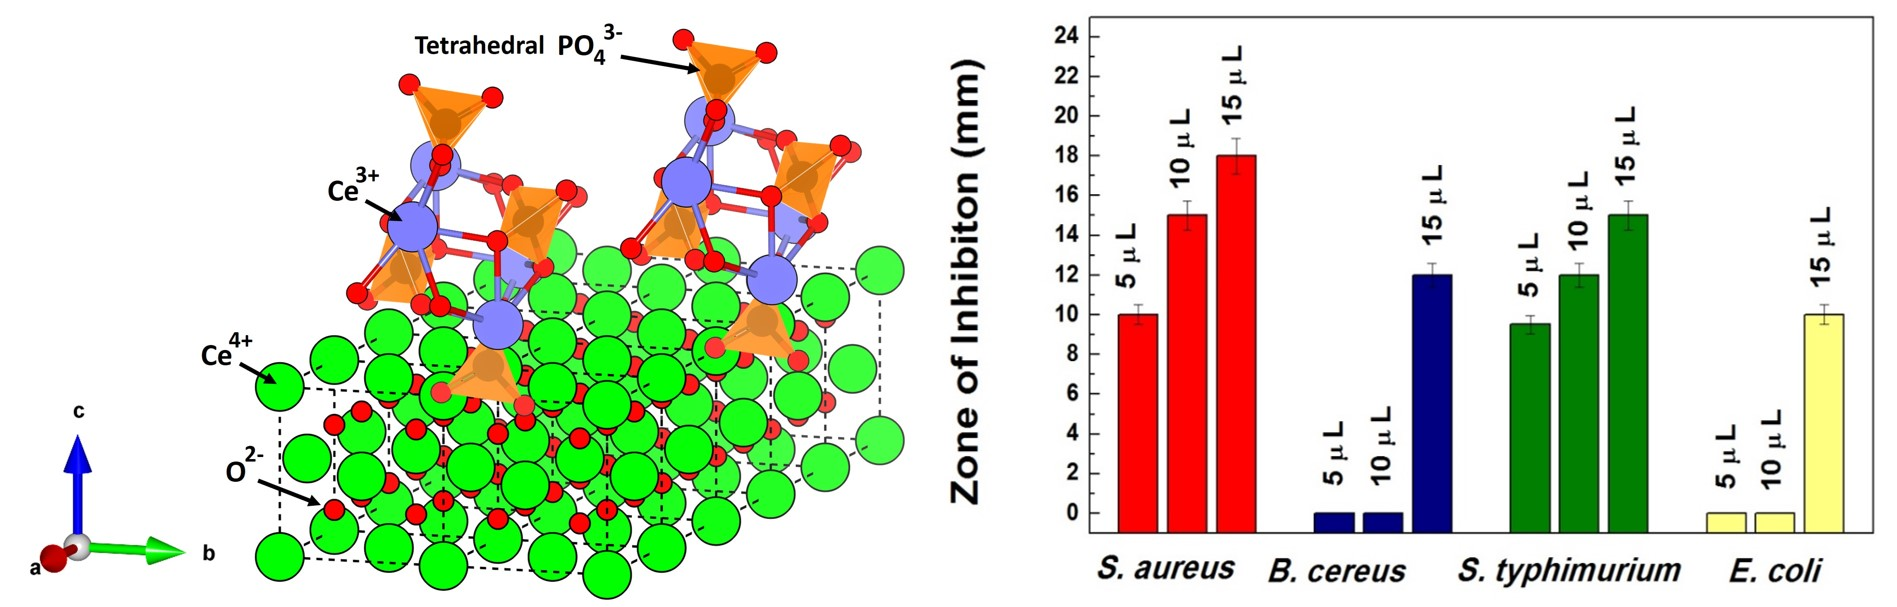
\includegraphics[width=0.98\linewidth]{Picture1}\\
    	\end{flushright}\end{minipage}

\vspace{20pt}    	 

%-----------paper-----------------
\section{\textbf{2. Amorphous interface oxide formed due to high amount of Sm doping (5-20 mol$\%$) stabilizes finer size anatase and lowers indirect band gap}}

\textbf{Authors:} Abdullah Zubair, \textbf{Abdullah Al Mamun}, Karrina McNamara, Syed AM Tofail, Fakhrul Islam, Vasily A Lebedev. \\ \vspace{3pt}

\textbf{Journal: Applied Surface Science, Elsevier, 2020} [link: https://doi.org/10.1016/j.apsusc.2020.146967] \\ \vspace{5pt}

    \begin{minipage}{.59\linewidth} \begin{flushleft}
    
    		\textbf{Abstract:} In this study, we have synthesized $Ti_{(1-x)}Sm_{x}O_{2} (x = 0-20\%)$ nanocomposites by adopting an aqueous sol-gel route. A two or multi-phase mixture of titania and samarium oxide could be expected as samarium added $>5\%$ may exceed its solubility limit in anatase. Surface and high-resolution characterization found Sm forming a predominantly thin amorphous layer that is not discernible in conventional transmission electron microscopy. The addition of Sm in such a high amount stabilizes formation of anatase phase of $TiO_2$. Importantly, we observe that the incorporation of such high amount of Sm in titania leads to a grain growth inhibition of anatase. Sm can also be reduced from a trivalent state to a bivalent state. The addition of Sm thus results in very thin amorphous layer around the nanocrystalline anatase, inhibits the growth of this anatase and lowers the indirect band gap from $3.0$ eV to $2.47$ eV. That such lowering happens along with a lowering of size and a resulting increase in surface area means that doping of titania by more than $5\%$ Sm can make better a photocatalyst either for the purpose of photodegradation of industrial organic water-pollutants and microorganisms under the visible light irradiation than a pristine anatase. 
    	\end{flushleft} \end{minipage}
    \hfill 
    \begin{minipage}{0.4\linewidth}\begin{flushright}
    	 	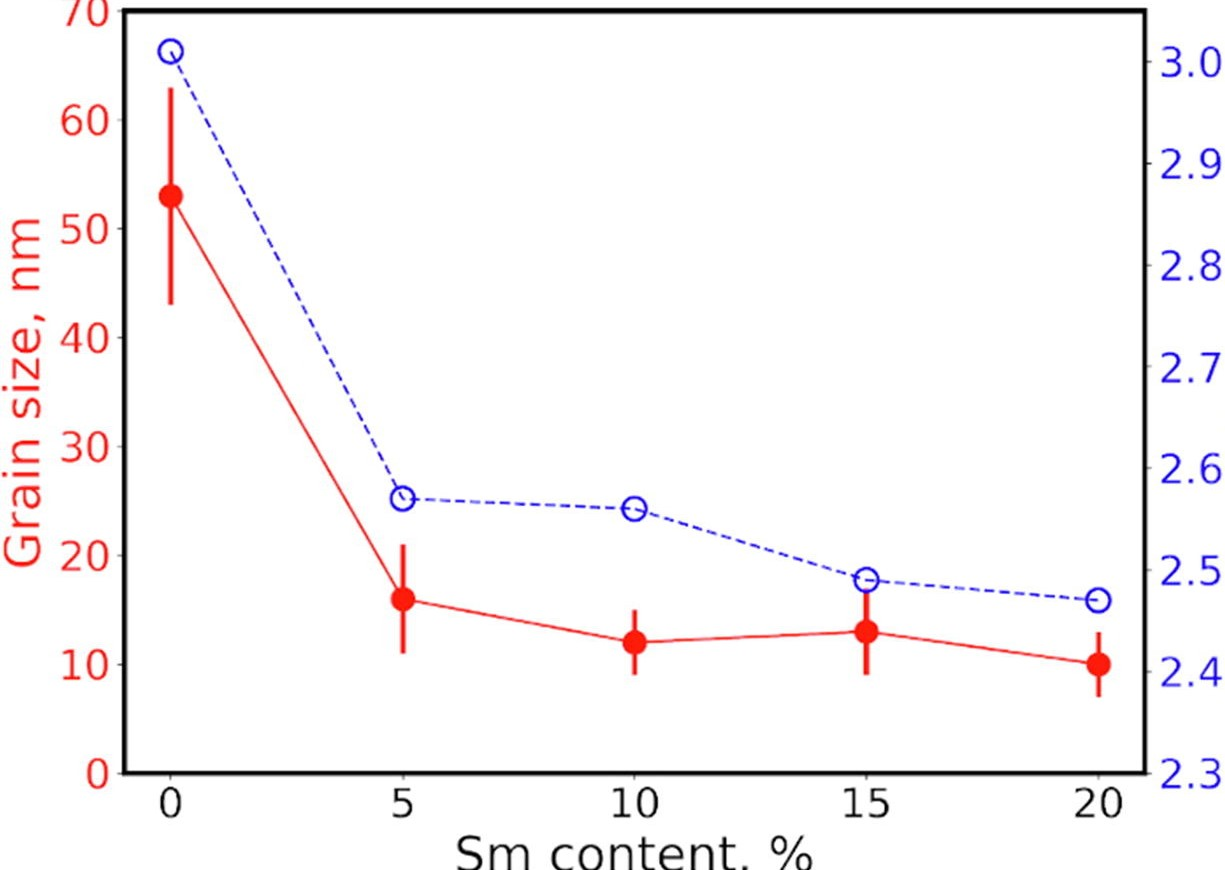
\includegraphics[width=0.80\linewidth]{AppSurf1}\\
    	 	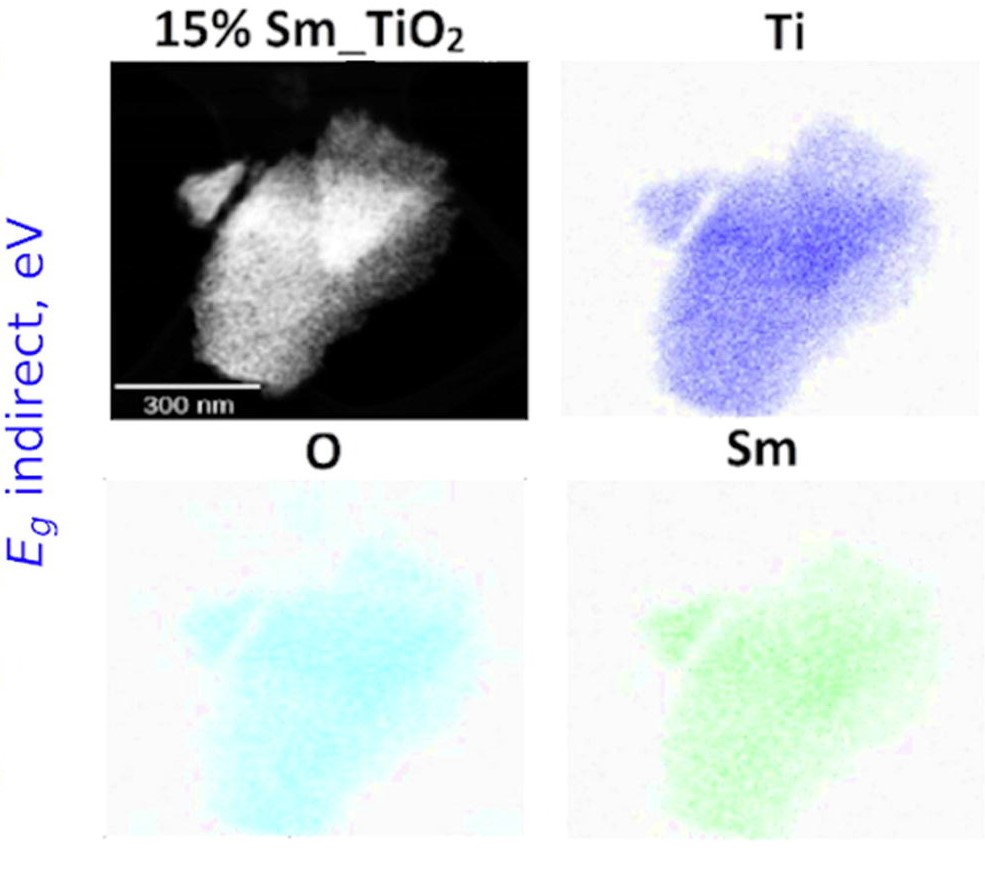
\includegraphics[width=0.8\linewidth]{AppSurf2}
    	\end{flushright}\end{minipage}
    	 
%-----------paper-----------------
\section{\textbf{3. Enhanced electrical conductivity and multiferroic property of cobalt‑doped bismuth ferrite nanoparticles}}

\textbf{Authors:} MM Rhaman, MA Matin, \textbf{MA Al Mamun}, A Hussain, MN Hossain, BC Das, MA Hakim, MF Islam. \\ \vspace{3pt}

\textbf{Journal: Journal of Materials Science: Materials in Electronics, Springer Nature} [link: https://doi.org/10.1007/s10854-020-03407-6] \\ \vspace{10pt}

\textbf{Abstract:} Multiferroic pure and cobalt-doped bismuth ferrite nanoparticles were synthesized by sol–gel method. The X-ray diffraction study showed a distinct crystalline phase with rhombohedral R3c structure. Rietveld refinement confirmed the reduction of crystallite size from 68 to 45 nm in doped BFO. Transmission electron microscopy \\ \vspace{2pt}

    \begin{minipage}{.59\linewidth} \begin{flushleft}
    
    	  was performed to confirm the morphology and lattice constant of the pure and cobalt-doped bismuth ferrite nanoparticles. The results of lattice constant have also been compared with the XRD results. Dielectric properties such as resistance, reactance, impedance, and resistivity were significantly decreased in doped BFO to 7.5 M$\Omega$, 14 M$\Omega$, 17 M$\Omega$, 3.7 M$\Omega$-m, respectively, at 100 Hz with concurrent increased conductivity of 0.184 (S/m)×${10}^{–3}$ at 10 MHz. The ferroelectric properties of pure and doped samples exhibited signifcantly enhanced maximum polarization and coercive feld in doped BFO of 16 µC/cm2 and 6.2 kV/cm, respectively, at an applied feld of 15 kV/cm. Ferromagnetic measurements of synthesized cobalt-doped BFO nanoparticles displayed a substantial improvement in saturation magnetization and coercive force of 7.07 emu/gm and 0.9 kOe, respectively. The important enhancement of magnetic properties with moderate value of coercive feld of the cobalt-doped samples may have potential applications in spintronics and memory devices.. 
    	\end{flushleft} \end{minipage}
    \hfill 
    \begin{minipage}{0.4\linewidth}\begin{flushright}
    	 	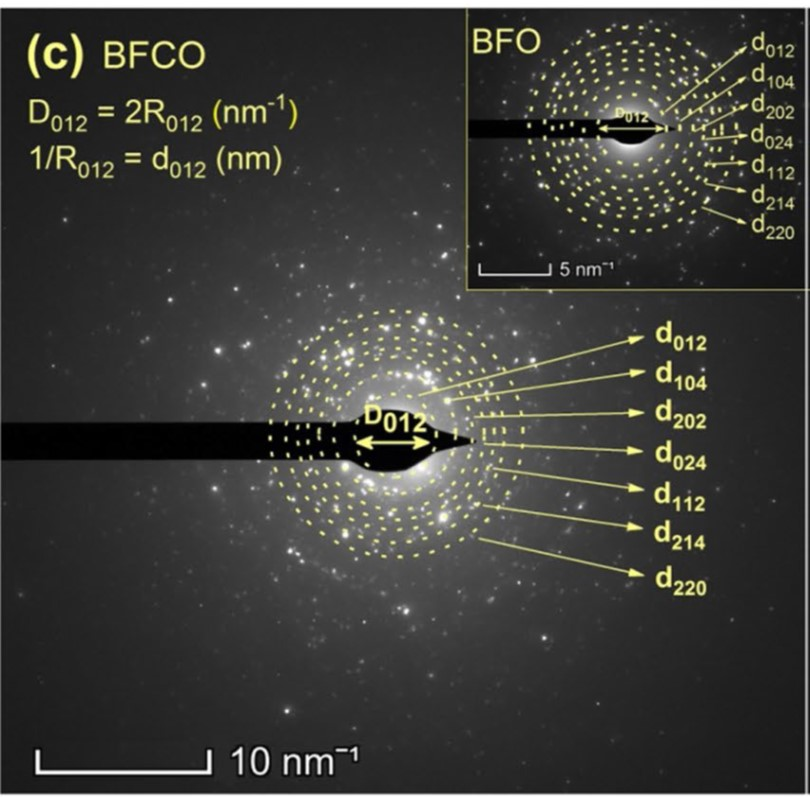
\includegraphics[width=0.85\linewidth]{jms}\\
    	 	
    	\end{flushright}\end{minipage}

\vspace{20pt}

%-----------paper-----------------
\section{\textbf{4. Nano-Porous Materials for Use in Solar Cells and Fuel Cells}}

\textbf{Authors:} \textbf{Md Abdullah Al Mamun}, Md Abdullah Al Mamun, Manifa Noor, Muhammad Hasanuzzaman, Saleem Hashmi. \\ \vspace{3pt}

\textbf{Book: Encyclopedia of Renewable and Sustainable Materials, Elsevier, Oxford 2020} [link: https://doi.org/10.1016/B978-0-12-803581-8.11267-6] \\ \vspace{8pt}

    \begin{minipage}{.98\linewidth} \begin{flushleft}
    
    		\textbf{Abstract:} The quest for efficient utilization of renewable energy and development of sustainable, green energy sources have gathered enormous interest among the researchers since last decade. Solar and fuel cells provide a key solution to conversion and storage of energy. In this review, we revisited the potential of porous Si (PSi) and Dye Sensitized Solar Cell (DSSC) for their unquestionable facile state-of-the-art fabrication techniques. Porosity is turned out to be a blessing in nanostructured Si solar cell as it can be used for anti-reflection coating to absorb more sunlight, trap the photons by improving internal reflection, and excellent reusable substrate to reduce the cost of wafer. On the other hand, fuel cell technology is dominant when efficient green energy is a priority. One of the major components of fuel cell is porous electrodes. Researchers emphasize more on developing porous electrodes in order to achieve higher efficiency at low temperature which leads to less greenhouse gas emission, durability, noise-free reliable source of power.
    	\end{flushleft} \end{minipage}

\vspace{5pt}

%-----------paper-----------------
\section{\textbf{5. An investigation of $^{60}Co$ gamma radiation-induced effects on the properties of nanostructured $\alpha-MoO_{3}$ for the application in optoelectronic and photonic devices}}

\textbf{Authors:} Sapan Kumar Sen, Manifa Noor, \textbf{MA Al Mamun}, M. S. Manir, M. A. Matin, M. A. Hakim, Salahuddin Nur, Supria Dutta. \\ \vspace{3pt}

\textbf{Journal: Optical and Quantum Electronics, 2019} [link: https://doi.org/10.1007/s11082-019-1797-9] \\ \vspace{-5pt}

    \begin{minipage}{.98\linewidth} \begin{flushleft}
    
    		\textbf{Abstract:} Gamma ray has sufficient energy to ionize and displace of atoms when interacts with optoelectronic and photonic devices that are placed at $\gamma$-radiation exposure environment, can be exposed to gamma radiation, resulting the alteration of the physical properties and hence the performances of devices. A comprehensive investigation of physical properties of the semiconductor materials under the influence of gamma radiation is essential for the effective design of devices for the application in the radiation exposure environment. In this article, a potential candidate for optoelectronic and photonic devices, orthorhombic $MoO_3$ nanoparticles with average crystallite size of 135.31 nm successfully synthesized by hydrothermal method. Then, the properties of nanoparticles exposed to low (10 kGy) and high (120 kGy) absorbed dose of $\gamma$-rays from $^{60}Co$ source were characterized by XRD, FESEM, FTIR and UV–Vis–NIR spectrophotometer and effects of absorbed doses was investigated for the first time. A significant change is observed in different physical properties of $\alpha-MoO_3$ nanoparticles after gamma exposure. The XRD patterns reveal the average crystallite size, intensity and the degree of crystallinity decrease for low dose (10 kGy) and increases for high dose (120 kGy). The calculated average crystallite size exposed to low and high doses are 127.79 nm and 136 nm, respectively. The lattice strain and dislocation density, however, shows the opposite trend of crystallite size with absorbed doses. This result is good evidence for the deterioration of crystallinity for low dose and improvement for high dose. The FESEM results reveal the significant effects of gamma doses on the micrographs of layered structure and on grain size. The optical studies disclose that band gap increases gradually from 2.78 to 2.90 eV, this behavior is associated with the reduction of electronic localized states. These results suggest that $\alpha-MoO_3$ nanoparticles could tolerate high doses of gamma radiation, making it a promising candidate for optoelectronic and photonic devices for $\gamma$-ray exposure environment applications.
    	\end{flushleft} \end{minipage}
    	
\vspace{7pt}

%-----------paper-----------------
\section{\textbf{6. Effect of $CePO_4$ on structural, magnetic and optical properties of ceria nanoparticles}}

\textbf{Authors:} \textbf{Md Abdullah Al Mamun}, Manifa Noor, AKM Atique Ullah, Md Sarowar Hossain, Matin Abdul, Fakhrul Islam, MA Hakim. \\ \vspace{3pt}

\textbf{Journal: Materials Research Express, 2018} [link: https://doi.org/10.1088/2053-1591/aae2d0] \\ \vspace{5pt}

    \begin{minipage}{.59\linewidth} \begin{flushleft}
    
    		\textbf{Abstract:} We report an intrinsic dilute ferromagnetism in $CeO_2$ nanoparticles prepared by a green synthesis route where Artocarpus Heterophyllus leaf extract is used as a bioreducing agent. ${{{\rm{PO}}}_{4}}^{3-}$ ions from leaf extract lock oxygen vacancy derived $Ce^{3+}$ ions as $CePO_4$ at surface of the $CeO_2$ nanoparticles. The observed ferromagnetic behavior is strongly influenced by the distribution of frustrated $Ce^{3+}$ ions at surface which has been attributed to the RKKY (Ruderman–Kittel–Kasuya–Yosida) type indirect exchange interaction of the spins. A giant redshift ($\sim$0.3 eV) in the optical bandgap with decrease in particle size indicates the presence of a spin polaron formed by the interaction between heavy fermion $\&$ charge carrier electrons in the system. The concept of locking the surface spins by phosphate ions may open up new possibilities for manipulation of the spin polarized charge carriers in future spintronics researches.
    	\end{flushleft} \end{minipage}
    \hfill 
    \begin{minipage}{0.4\linewidth}\begin{flushright}
    	 	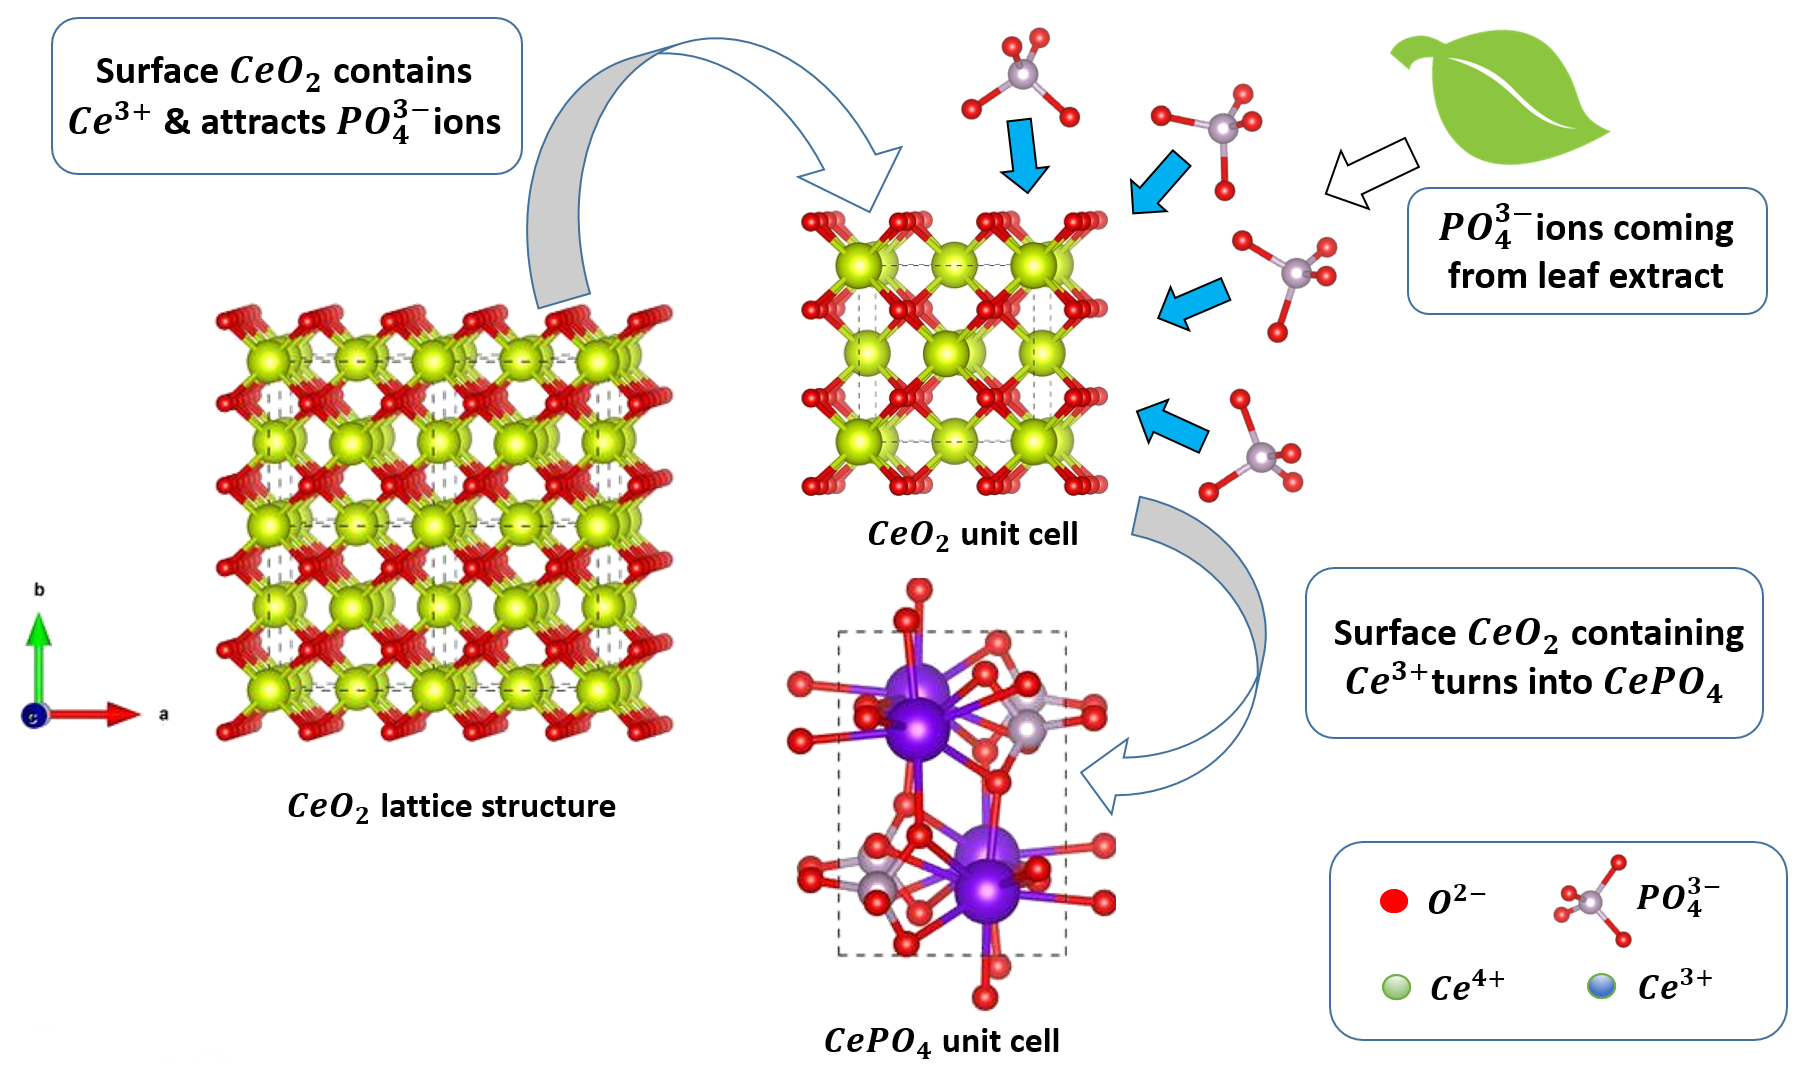
\includegraphics[width=1.0\linewidth]{mrx}\\
    	\end{flushright}\end{minipage}
    	 
\vspace{5pt}
%-----------paper-----------------
\section{\textbf{7. Effect of pH Variation on Structural, Optical and Shape Morphology of $BiVO_4$ Photocatalysts}}

\textbf{Authors:} Manifa Noor, \textbf{MA Al Mamun}, MA Matin, Md Fakhrul Islam, Saima Haque, Farabi Rahman, MN Hossain, MA Hakim \\ \vspace{3pt}

\textbf{Conference: $10^{th}$ International Conference on Electrical and Computer Engineering (ICECE), 2018} [link: https://doi.org/10.1109/ICECE.2018.8636721] \\ \vspace{5pt}

\textbf{Abstract:} Visible light driven photocatalysts have gathered enormous interest in recent years because of their capability to harvest energy directly from sunlight by water splitting and also to purify water. \\ \vspace{2pt} 

    \begin{minipage}{.69\linewidth} \begin{flushleft}
    
    		 Bismuth Vanadate (BVO) is one of the most potential photocatalysts for water pollutant degradation and hydrogen production by oxidation of water. In our study, highly crystalline Bismuth Vanadate nanoparticles have been synthesized by a straightforward hydrothermal route where pH is varied to observe the change in morphology of the particles. Thermal analysis confirmed the tetragonal to monoclinic phase transformation temperature at 350 $^{\circ}$C. A hierarchical development of monoclinic - tetragonal heterostructure of Bismuth Vanadate is further confirmed by Rietveld refinement of XRD patterns and the obtained particle size is 27nm. Band gap energy has been tailored through control of pH to explore the optical band gap for suitable photocatalytic properties. It is found that a heterostructure composed of rod and spherical shaped nanoparticles for a pH value 6.5, closer to neutral, demonstrating better optical properties for efficient photocatalytic activity with a band gap energy of 1.8 eV.
    	\end{flushleft} \end{minipage}
    	 \hfill 
    \begin{minipage}{0.29\linewidth}\begin{flushright}
    	 	
\includegraphics[width=1.0\linewidth]{ieee}\\
    	\end{flushright}\end{minipage}
    	
\vspace{8pt}


%-----------paper-----------------
\section{\textbf{8. Hydrothermal Synthesis and Characterization of Bismuth Vanadate Photocatalyst}}

\textbf{Authors:} \textbf{MA Al Mamun}, AFM Hossain, Miftaur Rahman, MH Rizvi. \\ \vspace{3pt}

\textbf{Conference: $1^{st}$ International Conference on Engineering Materials and
Metallurgical Engineering, BCSIR, 2016.} [link: www.icemme.com] \\ \vspace{5pt}

\textbf{Abstract:} Particulate photocatalyst for hydrogen production by water splitting and water purification has received a great attention because of their low cost and applicability in mass scale. Bismuth vanadate ($BiVO_4$) has recently emerged as one of the most promising photocatalysts for hydrogen production via water splitting and degradation of \\ \vspace{2pt}

    \begin{minipage}{.68\linewidth} \begin{flushleft}
    
    		pollutants. Based on previous studies, it’s well established that pure monoclinic (m)- $BiVO_4$ has showed the best photocatalytic performance so far. In this investigation, pure m-BiVO4 nanoparticles have been synthesized in a hydrothermal synthesis process: $(Bi(NO_{3})_{3}.5H_{2}O/V_{2}O_{5}/K_{2}SO_{4}, 200 ^{\circ} C)$. It is demonstrated that formation of pure m-BiVO4 with less impure phases is enhanced by addition of an inorganic morphology controlling agent $(K_{2}SO_{4})$ in system has been demonstrated. $Bi_{(1-x)}Nd{x}VO_{4}$ and $BiMn_{x}V_{(1-x)}O_{4}$ (where x = 0.10) nanoparticles have been synthesized to investigate the effects of doping on the structural formation, optical bandgap, particle size and morphology of particulate BiVO4. In $(Bi(NO_{3})_{3}.5H_{2}O/V_{2}O_{5}/K_{2}SO_{4}, 200 ^{\circ} C)$ system, $BiMn_{x}V_{(1-x)}O_{4}$ and $Bi_{(1-x)}Nd{x}VO_{4}$ were formed as pure m-$BiVO_4$ and a small presence of zircon type $BiVO_4$ was found in $Bi_{(1-x)}Nd{x}VO_{4}$ (where x = 0.10). The reason of a slight increase in bandgap energy of $Bi_{(1-x)}Nd{x}VO_{4}$ (where x = 0.10) has also been explained. In future, the synthesized bismuth vanadate nanoparticles will be used for photocatalytic degradation of dyes.
    	\end{flushleft} \end{minipage}
    	\hfill 
    \begin{minipage}{0.29\linewidth}\begin{flushright}
    	 	
\includegraphics[width=1.0\linewidth]{icemme}\\
    	\end{flushright}\end{minipage}

\end{document}



